\documentclass[../lecture1-introduction.tex]{subfiles}

\begin{document}

\section{Editing, Compiling, and Execution}
% http://www-h.eng.cam.ac.uk/help/languages/C++/c++_tutorial/editing.html
% -------------------------------------------------------------------

\begin{frame}[fragile]{A Simple Program to Add Two Numbers}
    The following is an example of a simple program written in C++.
\begin{cppcode}[]
#include <iostream>
using namespace std;

int main()
{
    int num1, num2, total;

    cout << "Enter integers to be added:" << endl;
    cin >> num1 >> num2;
    total = num1 + num2;
    cout << "The sum is " << total << endl;

    return 0;
}
\end{cppcode}
    \only<1>
    {
        I double dare you to guess what this program does.
    }
    \only<2>
    {
        This program is designed to read two numbers typed by the user at the
        keyboard; Compute their sum and display the result on the screen.
    }
    \only<3>
    {
        What could we do to make understanding this program easier?
    }
\end{frame}

% -------------------------------------------------------------------

\begin{frame}[fragile]{A Simple Program with Comments}
    Add comments!
\begin{cppcode}[]
// Program to add two integers typed by user at keyboard
#include <iostream>
using namespace std;

int main()
{
    int num1, num2, total;

    cout << "Enter integers to be added:" << endl;
    cin >> num1 >> num2;
    total = num1 + num2;
    cout << "The sum is " << total << endl;

    return 0;
}
\end{cppcode}
\end{frame}

% -------------------------------------------------------------------

\begin{frame}[fragile]{A Not So Simple Program Because OMG Whoever Wrote This Is An \tiny{ass}}
    Or hey, if you want to guarantee yourself a job
\begin{cppcode}[]
#include <iostream>
using namespace std;
int main(){
    int n,b,memes = 42;
cout<<"gimmie:" <<endl;
        cin>>n>>b;
    memes=n+b;
cout<<"got em" <<memes+1-1<<endl;
    return (pow(meme, 0) - 1);}
\end{cppcode}
\end{frame}

% -------------------------------------------------------------------

\begin{frame}[fragile]{Program Structure and Syntax}
    C++ uses notation that may appear strange to non-programmers (and me).
    The notation is part of the programming language \texttt{syntax}.
    \begin{description}
        \item [Syntax] Formal rules that specify the structure of a legal program.
    \end{description}
\end{frame}

\begin{frame}[fragile]{Program Structure and Syntax}
    The notation and explanations which follow will appear strange if you have
    never written a computer program. \newline \newline
    Don't worry about them or how the program works. This will be explained
    in more detail later. \newline \newline
    The following is an overview.
\end{frame}

\begin{frame}[fragile]{Program Structure and Syntax}
    Every C++ program consists of a header and a main body and has the following
    structure:
\begin{cppcode}[]
// Comment statements which are ignored by computer
/* Also a comment */
#include < header file name >

int main()
{
    declaration of variables;
    statements;

    return 0;
}
\end{cppcode}
\end{frame}

\begin{frame}[fragile]{Program Structure and Syntax}
\begin{cppcode}[]
// Program to add two integers typed by user at keyboard
#include <iostream>
using namespace std;

int main()
{
    int num1, num2, total;

    cout << "Enter integers to be added:" << endl;
    cin >> num1 >> num2;
    total = num1 + num2;
    cout << "The sum is " << total << endl;

    return 0;
}
\end{cppcode}
    \only<1>
    {
        Line 1
        \begin{itemize}
            \item Lines beginning with // indicate that the rest of the line
            is a \textbf{comment}.
            \item Comments are inserted by programmers to help people read
            and understand the program.
            \item Can be placed anywhere in a program.
        \end{itemize}
    }
    \only<2>
    {
        Line 2
        \begin{itemize}
            \item Lines beginning with \# are instructions to the compiler's
            preprocessor.
            \item The \textbf{include} instruction says "what follows is a file name,
            find that file and insert its contents right here".
            \item Here the file iostream contains the definitions of
            \textbf{cin}, \textbf{cout}.
        \end{itemize}
    }
    \only<3>
    {
        Line 3
        \begin{itemize}
            \item Specifies that names used in the program (ie. \textbf{cin} and
            \textbf{cout}) are defined in the standard libraries.
            \item This is used to avoid problems with other libraries which may
            also use these names.
        \end{itemize}
    }
    \only<4>
    {
        Line 5
        \begin{itemize}
            \item When the program is executed the instructions will be executed
            in the oder they appear in the main body of the program.
            \item The main body is delimited by main() and the curly braces \{ \}.
            \item This line also specifies that main() will return a value of type
            integer (int) on its completion (see line 14).
        \end{itemize}
    }
    \only<5>
    {
        Line 6
        \begin{itemize}
            \item The opening (left) brace marks the beginning of the main body
            of the program.
            \item The main body consists of instructions which are \textbf{declarations}
            defining the data or \textbf{statements} on how the data should be
            processed.
            \item All C++ declarations and statements must end with a semicolon;
        \end{itemize}
    }
    \only<6>
    {
        Line 7
        \begin{itemize}
            \item This is a declaration. The words num1 and num2 are the names
            of \textbf{variables}.
            \item A variable is a location in the computer's memory where a value
            can be stored for use by a program.
            \item The declaration also specifies the variable \textbf{type}
        \end{itemize}
    }
    \only<7>
    {
        Line 9
        \begin{itemize}
            \item This statement instructs the computer to output the \texttt{string}
            of characters contained between the quotation marks, followed by a
            new line \textbf{endl}.
            \item The location of the output is denoted by \textbf{cout} which in this
            case will be the terminal screen.
        \end{itemize}
    }
    \only<8>
    {
        Line 10
        \begin{itemize}
            \item This statement instructs the computer to read data typed in at
            the keyboard (standard input), denoted by \textbf{cin}.
            \item These values are \texttt{assigned to} (stored in) variables num1
            and num2.
        \end{itemize}
    }
    \only<9>
    {
        Line 11
        \begin{itemize}
            \item This statement is an \textbf{arithmetic expression} which assigns
            the value of the expression num1 + num2 (sum of integer values stored
            at num1 and num2) to the variable total.
        \end{itemize}
    }
    \only<10>
    {
        Line 12
        \begin{itemize}
            \item Instructs the computer to display the value of the variable total.
        \end{itemize}
    }
    \only<11>
    {
        Line 14
        \begin{itemize}
            \item The last instruction of every program is the return statement.
            \item The return statement with the int value 0 (zero) indicates to
            the operating system that the program has terminated successfully.
        \end{itemize}
    }
    \only<12>
    {
        Line 15
        \begin{itemize}
            \item The closing (right) brace marks the end of the main body of
            the program.
        \end{itemize}
    }
    \only<13>
    {
        Blank lines
        \begin{itemize}
            \item Lines 4, 8 and 13 are used to make the program more readable.
            \item They will be ignore by the compiler.
            \item \textbf{Whitespace} (spaces, tabs and newlines) are also ignored
            (unless within quotation marks).
        \end{itemize}
    }
    \only<14>
    {
        Indentation
        \begin{itemize}
            \item It does not matter where you place statements, either on the
            same line or on separate lines.
        \end{itemize}
    }
\end{frame}

% -------------------------------------------------------------------

\begin{frame}[fragile]{Development Environment \& Development Cycle}
    C++ programs go through 3 main phases during development:
    \begin{description}
        \item [Editing] Writing the program,
        \item [Compiling] Translating the program to executable code and detecting
        syntax errors, and
        \item [Debugging] Running the program and checking for logical errors.
    \end{description}
\end{frame}

% -------------------------------------------------------------------

\begin{frame}[fragile]{Check this out}
    \begin{center}
        \makebox[\textwidth]{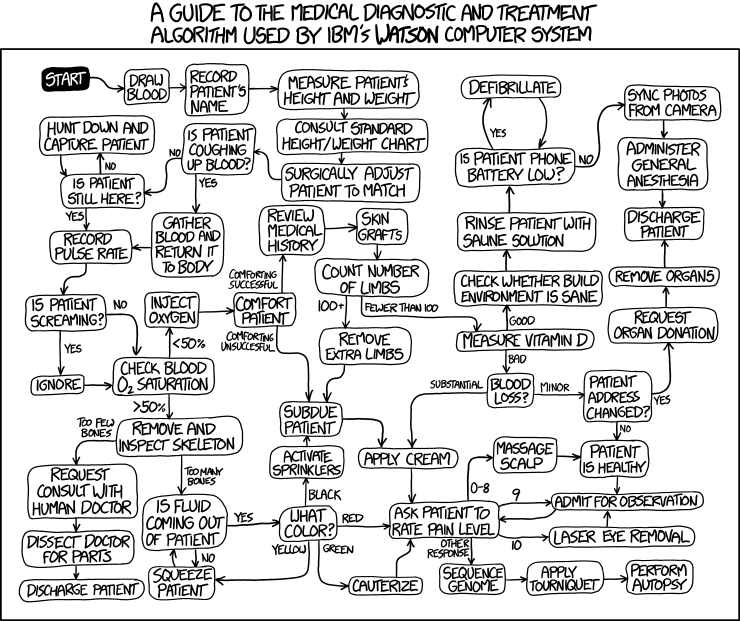
\includegraphics[width=\paperwidth,height=\textheight,keepaspectratio]{graphics/xkcd1619-watson_medical_algorithm.png}}
    \end{center}
\end{frame}

% -------------------------------------------------------------------

\end{document}
